\documentclass[a4paper]{article}
\usepackage[utf8]{inputenc}
\usepackage[T1]{fontenc}
\usepackage{graphics}
\usepackage{libertine}
\usepackage{tango}
%\usepackage[colorlinks=true]{hyperref}

\hypersetup{urlcolor=DarkChocolate}

\title{Mémo Git}
%\author{\scalebox{0.35}{ \includegraphics{logo_azae}}}
\author{Thomas Clavier}
\date{}

\setlength{\parindent}{0pt}
\newcounter{question}
\setcounter{question}{1}
\newcommand{\q}{
  \textcolor{DarkOrange}{\textbf{Question \thequestion : }}
  \addtocounter{question}{1}
  \newline
}

\begin{document}

\maketitle

\section*{Présentation}

Git est un logiciel de gestion de versions décentralisé.

Ce mémo est un extrait du livre : \url{https://git-scm.com/book/fr}

\subsection*{Des objets}
Un dépôt Git peut être vu comme une collection d’objets liés entre eux. 
Chaque objet est identifié par une chaîne de 40 caractères hexadécimaux
correspondant à la somme de contrôle de son contenu. 
Il y a 3 types d'objets : 
\begin{itemize}
\item blob : les données
\item tree : les arborescences
\item commit : une version du répertoire de travail
\end{itemize}
Un objet de type <<arborescence>> peut contenir des objets <<données>> et <<arborescence>>.
Le répertoire de travail est lui-même un objet de type <<arborescences>>. 

L'historique d'un dépôt Git c'est l'ensemble des versions du répertoire de travail. Pour identifier une version, Git s'appuie sur un objet de type <<commit>>. 
L'objet de type <<commit>> associe de nombreuses informations comme l'auteur, un message, une version de l'objet répertoire de travail mais aussi les <<commits> parents.

\begin{figure}[h]
  \center
  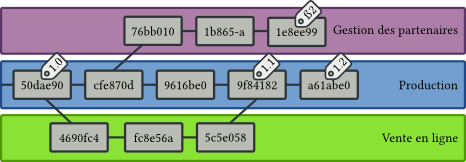
\includegraphics{graphs}
  \caption{Historiques de commits}
\end{figure}
%TODO 3 schémas : graph de versions (branches) graphs de commits et tree + blob

\subsection*{Les espaces}
Git utilise 3 espaces différents pour manipuler toutes ces données.
\begin{itemize}
\item le répertoire de travail
\item l'index
\item l'historique
\end{itemize}

Le répertoire de travail présente dans un dossier de la machine, l'ensemble des fichiers du dépôt. C'est le point d'entrée de l'utilisateur.

L'index contient les données en préparation pour le commit

La tête (HEAD) de l'historique contient le dernier commit.

\begin{figure}[h]
  \center
  \scalebox{0.7}{ 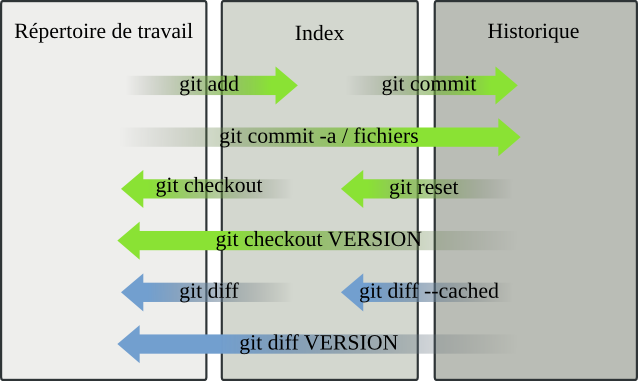
\includegraphics{espaces}}
  \caption{3 espaces de données}
\end{figure}

\subsection*{À distance}
Avec les commandes push, pull et fetch, il est possible d'envoyer ou de recevoir la totalité de l'historique d'une branche vers un serveur distant. Ce qui permet de travailler à plusieurs sur le même projet.

\vspace{2mm}

\begin{figure}[h]
  \center
  \scalebox{0.7}{ 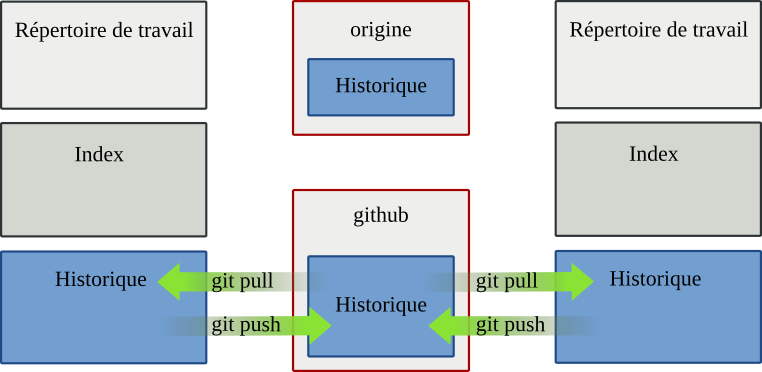
\includegraphics{remote}}
  \caption{Serveurs distants}
\end{figure}

\section*{Resources}
Pour avoir de l'aide sur git, il est possible de lancer "man git". Pour
avoir de l'aide sur la commande "git log" il est possible de lancer "man
git-log".

\section*{Principales commandes}

Toutes les commandes git sont de la forme suivante : 
\begin{verbatim}
git action [options] argument
\end{verbatim}

\subsection*{config}

Permet de configurer les variables de paramétrage de git

L'option \textit{global} permet de configurer les variables de l'utilisateur, donc valable pour l'ensemble des projets de l'utilisateur.

L'option \textit{system} permet de configurer les variables de tous les utilisateurs.

\begin{verbatim}
git config --global user.name "Thomas Clavier"
\end{verbatim}

\subsection*{init}

Initialiser un répertoire de travail comme un dépôt local git. Permet d'initialiser l'ensemble des 3 espaces.

Exemple pour le répertoire courant : 
\begin{verbatim}
git init .
\end{verbatim}

\subsection*{add}
Ajouter un fichier à suivre dans l'index. Pour préparer un commit.
\begin{verbatim}
git add chemin/vers/fichier
\end{verbatim}

\subsection*{commit}
Valider l'index actuel pour créer un commit
\begin{verbatim}
git commit -m "Mon message de commit"
\end{verbatim}

\subsection*{log}
Observer l'historique des changements
\begin{verbatim}
git log
\end{verbatim}

\subsection*{diff}
Observer la différence entre 2 commits, permet par exemple de voir quelles sont les différences entre 2 commits sur un fichier donné.

\begin{verbatim}
git diff
\end{verbatim}

\subsection*{status}
Observer l'état de l'index et du répertoire de travail
\begin{verbatim}
git status
\end{verbatim}

\subsection*{rm}
Supprimer un fichier de l'index
\begin{verbatim}
git rm chemin/vers/fichier
\end{verbatim}

\subsection*{mv}
Déplacer un fichier. C'est équivalent à copier le fichier puis supprimer le fichier d'origine.
\begin{verbatim}
git mv chemin/vers/fichier chemin/vers/nouveau/fichier
\end{verbatim}

\subsection*{remote}
Permet de manipuler les adresses des adresses des index distants.
\begin{verbatim}
git remote add origin https://github.com/tclavier/tp-git-blog.git
\end{verbatim}

\subsection*{push}
Permet d'envoyer une copie de l'index des changements vers un serveur distant
\begin{verbatim}
git push origin master
\end{verbatim}

\subsection*{pull}
Permet de recevoir une copie de l'index d'un serveur distant
\begin{verbatim}
git pull origin master
\end{verbatim}

\subsection*{clone}
Prépare une copie de travail depuis un serveur distant
\begin{verbatim}
git clone URL
\end{verbatim}

\subsection*{clean}
Supprime les fichiers non suivis par git
\begin{verbatim}
git clean -f
\end{verbatim}

\subsection*{tag}
Permet de poser une étiquette sur un commit donné.
\begin{verbatim}
git tag 1.0.0
\end{verbatim}

\subsection*{merge}
Fusionne 2 branches.
\begin{verbatim}
git merge ma-branche
\end{verbatim}

\subsection*{rebase}
Concatène 2 branches.
\begin{verbatim}
git rebase ma-branche
\end{verbatim}

\subsection*{branch}
Crée un branche de travail
\begin{verbatim}
git branch ma-branch
\end{verbatim}

\subsection*{checkout}
Change la version de travail par une branche ou les fichiers du dernier commit
\begin{verbatim}
git checkout ma-branch
\end{verbatim}

\subsection*{cherry-pick}
Permet de prendre un commit quelconque et de l'appliquer localement.

Exemple : 
\begin{verbatim}
git cherry-pick ma-branche
\end{verbatim}
Permet d'appliquer le dernier commit de la branche <<ma-branche>> dans la branche courante.

\section{Fichiers particulier}

\subsection*{.gitignore}
Liste des fichiers ou répertoires que git doit ignorer

\subsection*{revert}
Crée un patch de retour en arrière affin d'annuler certains commits.

\begin{verbatim}
git revert HEAD~3
\end{verbatim}
Va créer un patch pour annuler les 4 derniers commits.


\end{document}

